\documentclass[tikz,border=8pt]{standalone}
\usepackage[T1]{fontenc}
\usepackage[utf8]{inputenc}
\usepackage{lmodern}
\usetikzlibrary{shapes.geometric,positioning}

\tikzset{
  every node/.style={font=\sffamily\fontsize{8.4}{9.6}\selectfont},
  usecase/.style={
    ellipse,
    draw=black,
    line width=0.65pt,
    minimum height=0.84cm,
    minimum width=3.55cm,
    text width=3.05cm,
    align=center,
    inner xsep=7pt,
    fill=white
  },
  association/.style={draw=black,line width=0.58pt}
}

\newcommand{\actor}[3]{%
  \coordinate (#1) at (#2,#3);
  \draw[line width=0.72pt] (#2,#3+0.42) circle (0.18);
  \draw[line width=0.72pt] (#2,#3+0.24) -- (#2,#3-0.25);
  \draw[line width=0.72pt] (#2-0.30,#3+0.05) -- (#2,#3+0.13) -- (#2+0.30,#3+0.05);
  \draw[line width=0.72pt] (#2,#3-0.25) -- (#2-0.27,#3-0.62);
  \draw[line width=0.72pt] (#2,#3-0.25) -- (#2+0.27,#3-0.62);
}

\begin{document}
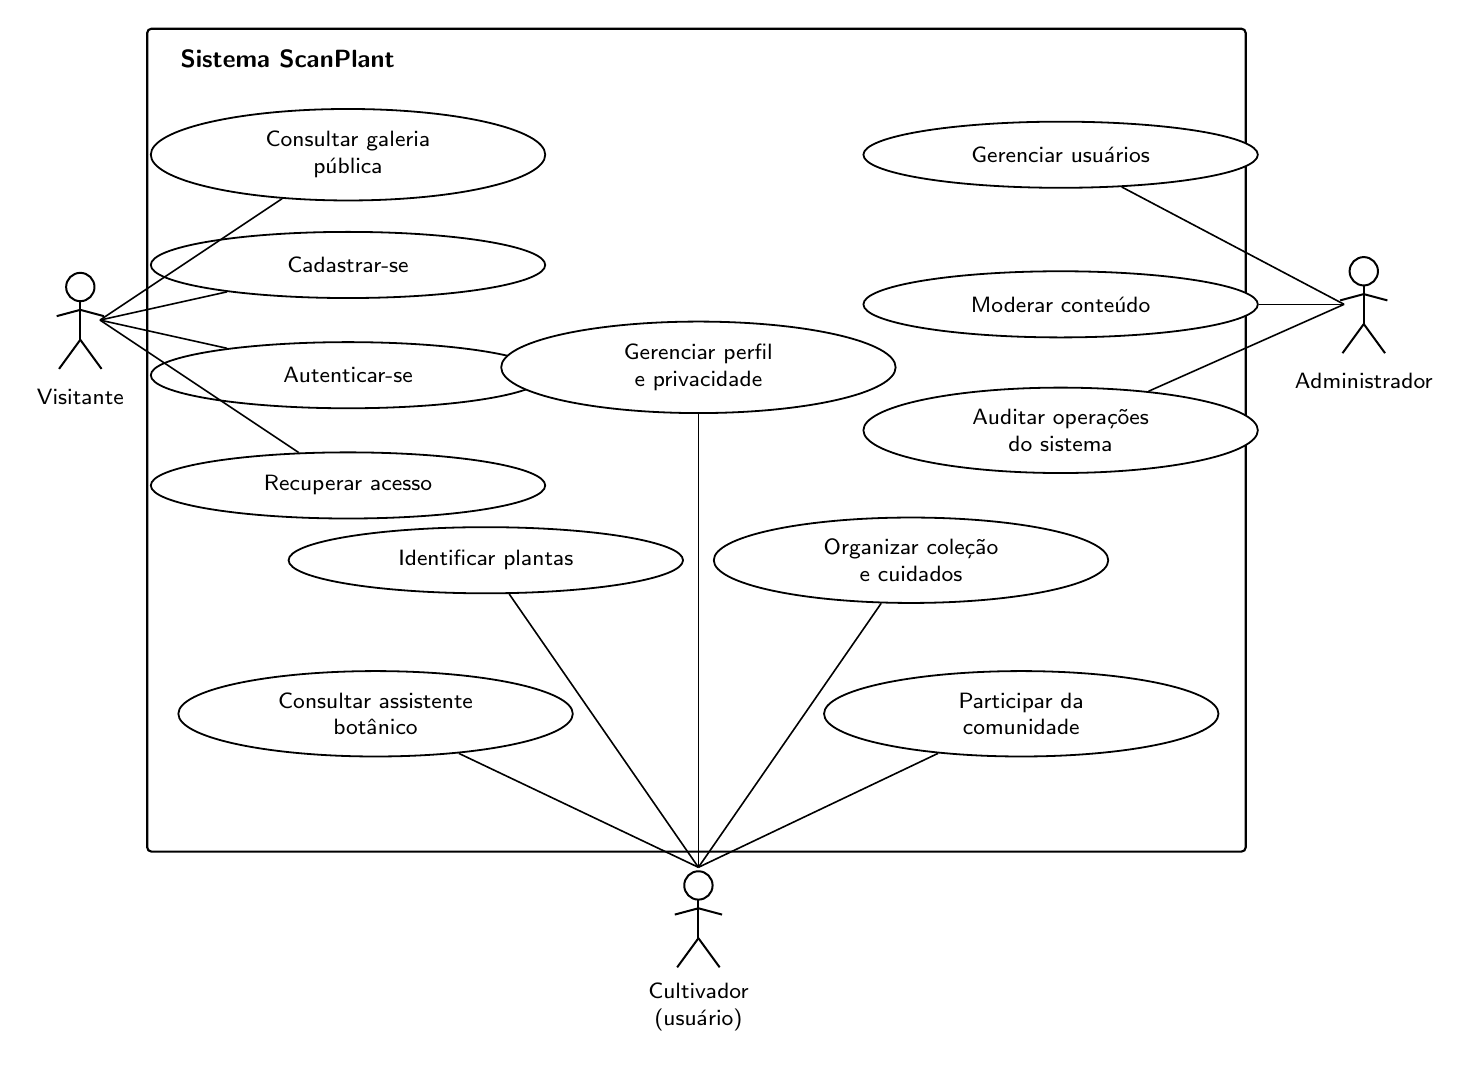
\begin{tikzpicture}
  % Limite do sistema: apenas os serviços observáveis ficam dentro dele.
  \draw[line width=0.78pt,rounded corners=1.5pt] (2.05,0.40) rectangle (16.00,10.85);
  \node[anchor=north west,font=\sffamily\bfseries\fontsize{9.2}{10.5}\selectfont]
    at (2.35,10.70) {Sistema ScanPlant};

  % Casos de uso do visitante.
  \node[usecase] (galeria) at (4.60,9.25) {Consultar galeria\\pública};
  \node[usecase] (cadastro) at (4.60,7.85) {Cadastrar-se};
  \node[usecase] (autenticar) at (4.60,6.45) {Autenticar-se};
  \node[usecase] (recuperar) at (4.60,5.05) {Recuperar acesso};

  % Casos de uso do cultivador: objetivos, não rotinas internas.
  \node[usecase,minimum width=3.85cm] (identificar) at (6.35,4.10)
    {Identificar plantas};
  \node[usecase,minimum width=3.85cm] (colecao) at (11.75,4.10)
    {Organizar coleção\\e cuidados};
  \node[usecase,minimum width=3.85cm] (assistente) at (4.95,2.15)
    {Consultar assistente\\botânico};
  \node[usecase,minimum width=3.85cm] (comunidade) at (13.15,2.15)
    {Participar da\\comunidade};
  \node[usecase,minimum width=3.85cm] (perfil) at (9.05,6.55)
    {Gerenciar perfil\\e privacidade};

  % Casos de uso administrativos.
  \node[usecase] (usuarios) at (13.65,9.25) {Gerenciar usuários};
  \node[usecase] (moderar) at (13.65,7.35) {Moderar conteúdo};
  \node[usecase,minimum width=3.85cm] (auditar) at (13.65,5.75)
    {Auditar operações\\do sistema};

  % Pontos de conexão dos atores, posicionados fora do limite do sistema.
  \coordinate (visitante-link) at (1.45,7.15);
  \coordinate (cultivador-link) at (9.05,0.20);
  \coordinate (administrador-link) at (17.25,7.35);

  % Associações simples. Relações de implementação e APIs não pertencem à visão geral.
  \foreach \uc in {galeria,cadastro,autenticar,recuperar}
    \draw[association] (visitante-link) -- (\uc);
  \foreach \uc in {identificar,colecao,assistente,comunidade,perfil}
    \draw[association] (cultivador-link) -- (\uc);
  \foreach \uc in {usuarios,moderar,auditar}
    \draw[association] (administrador-link) -- (\uc);

  % Atores UML.
  \actor{visitante}{1.20}{7.15}
  \node[align=center,anchor=north] at (1.20,6.40) {Visitante};

  \actor{cultivador}{9.05}{-0.45}
  \node[align=center,anchor=north] at (9.05,-1.15) {Cultivador\\(usuário)};

  \actor{administrador}{17.50}{7.35}
  \node[align=center,anchor=north] at (17.50,6.60) {Administrador};
\end{tikzpicture}
\end{document}
